\documentclass[12pt, a4paper]{article}
\usepackage[margin=2.0cm]{geometry}
\usepackage{stmaryrd}
\usepackage{amsmath}
\usepackage{amssymb}
\usepackage{enumerate}
\usepackage{bbold}
\usepackage{dsfont}
\usepackage{algorithm2e}
\usepackage{changepage}
\usepackage{undertilde}
\usepackage{hyperref}
\hypersetup{pdftex,colorlinks=true,allcolors=blue}
\usepackage{hypcap}
\usepackage{fancyhdr}
\usepackage{float}
\usepackage[english]{babel}
\usepackage{graphicx}
\usepackage{caption}
\usepackage{subcaption}
\usepackage{wrapfig}
\usepackage{multicol}

\pagestyle{fancy}
\fancyhf{}
\lhead{dc14770, rk14842}
\rhead{ML CW}

\setlength{\parskip}{.1in}
\setlength{\parindent}{0in}
\setlength{\columnsep}{0.5cm}

\begin{document}

	\begin{center}
	{ \Large \bf Introduction to Machine Learning }

  \end{center}
  \begin{center}
    \vspace{.1in}

    Spam Filter Coursework Report

    Dylan Cope and Rowan Kypreos

	\vspace{.2in}

	\end{center}

  \section{Simple Naive Bayes}

  \subsection{Constructing the Model} \label{classconstr}

  % \begin{multicols}{2}

  To prepare the data for a Naive Bayes model boolean features needed to be extracted from the emails. First the emails were preprocessed by splitting the text by whitespace and filtering out any strings that aren't composed purely of alphabetical characters. Next a list of words needed to be determined for a feature extraction process that checked the presence of a word in a email. In constructing this model a process for extracting feature words from the training set needs be provided. The primary reason for including the extraction process here is to ensure the feature words are determined purely from the training data, if the words were chosen from the entire available set of emails any scoring of the classifier would be invalid as it would be impossible to tell if the model had overfit.

  The Naive Bayes classifier for is defined by two estimator vectors $\utilde{\hat{\theta}}_s$ and $\utilde{\hat{\theta}}_h$ corresponding to spam and ham. Each element in the vectors then corresponds to a probability associated with the presence of a feature word. To tune the classifier's estimators the training emails $E$ are transformed to a matrix $X$ where each column corresponds to a feature word and each row corresponds to an email. The value of each entry in $X$ is either a 1 or a 0 depending on if the word for the column is in the email for the row. The rows of $X$ are then grouped by class and summated down the columns. The resultant bit vectors are then divided by the number of instances in that class to give the final estimator vectors with elements of the form,
  $$ \hat{\theta}_i = \frac{x_i}{N} $$
  where $x_i$ are the observations and $N$ is the number of trials.

  So far what been described is a simple Naive Bayes model with no smoothing. The implemented spam filter uses additive smoothing to allow the assignment of non-zero probabilities to words which do not occur in the sample. This changes the class estimators to be of the form,
  $$ \hat{\theta}_i = \frac{x_i + \alpha}{N + \alpha d} $$
  where $\alpha$ is the smoothing parameter and $d$ is the number of features.

  Finally with the tuned estimators a decision rule is determined for classifying future data. Given an observation $\utilde{x}$ and class priors $p$ and $(1-p)$ for ham and spam respectively we can define a classification function $C$,

  $$
    C(\utilde{x}) = \begin{cases}
      \text{ham} & \text{if } p P(\utilde{x}|\utilde{\hat{\theta}}_h) > (1-p) P(\utilde{x}|\utilde{\hat{\theta}}_s) \\
      \text{spam}  & \text{otherwise}
    \end{cases}
  $$

  Through assuming the observations are probabilistically independent the values $P(\utilde{x}|\utilde{\hat{\theta}})$ can be computed by multiplying together the elements $\utilde{\hat{\theta}}$ that correspond to true values in $\utilde{x}$.

  % \end{multicols}

  \subsection{Cross-Validation Scoring}

  Overfitting can occur by learning model parameters on the same data that's used for testing. A common solution to this is to partition the data into training and testing splits, however when evaluating across a models hyperparameter space there is still a risk of overfitting as the parameters will be tweaked to optimal performance.

  This leads to the idea of splitting the data three ways; testing, training and validation sets. The model's parameters can be tuned on the training set, the hyperparameters can be optimised on the validation set, then the final model can be assessed on the testing set. However splitting the data three ways means we drastically reduce the number of samples that can be used for learning the model, and the results can depend on the particular random choices made to split the data.

  This is solved with cross-validation (CV), a test set is still held out for final evaluation, but the validation set is no longer needed when doing CV. In the basic approach, called $k$-fold CV, the training set is split into $k$ smaller sets. A model is then trained using $k-1$ of the folds and validating on the remaining fold. This process is then repeated $k$ times with differing splits on the folds, and the procedure returns a list of $k$ mean accuracy scores from each trained model. From this list an overall mean score can be determined with a margin of error.

  \subsection{Comparing to a Baseline} \label{baseline}

  With the methodology for constructing and scoring classifiers determined, a baseline needed to be established to ensure the trained models are statistically significantly better at classifying the data. A classifier that makes predictions by randomly assigning classes obtains an accuracy of 0.5, while this is an acceptable baseline making assessments it doesn't reflect the class proportionality of the data. Instead we consider a classifier that always predicts the majority class, as the data is 80\% ham and 20\% spam, this classifier always predicts ham and has an accuracy of 0.8.

  In section \ref{classconstr} the method for constructing a model was details. The construction required a given feature word extraction process and hyperparameters for smoothing $\alpha$ and class priors $p$. Finding optimal hyperparameters for the classifier will be discussed in section \ref{hyperopt}, for now we follow Laplace's rule of sucession, i.e. $\alpha = 1$, and we let the class prior have no influence, i.e. $p = 0.5$.

  A simple feature words extraction process was be provided to the constructor whereby $n$ random words from the training set were taken as feature words.
  % In doing so the resultant classifier achieved a mean 5-fold cross-validation score of 88.0\% with a 0.7\% margin of error.

  % Now that the process for constructing and scoring classifiers has been established we can experiment with taking the $n$ words with the highest $d$ values.

  \begin{figure}[H]
    \caption{Number of features against performance}
    \label{numfeatures}
    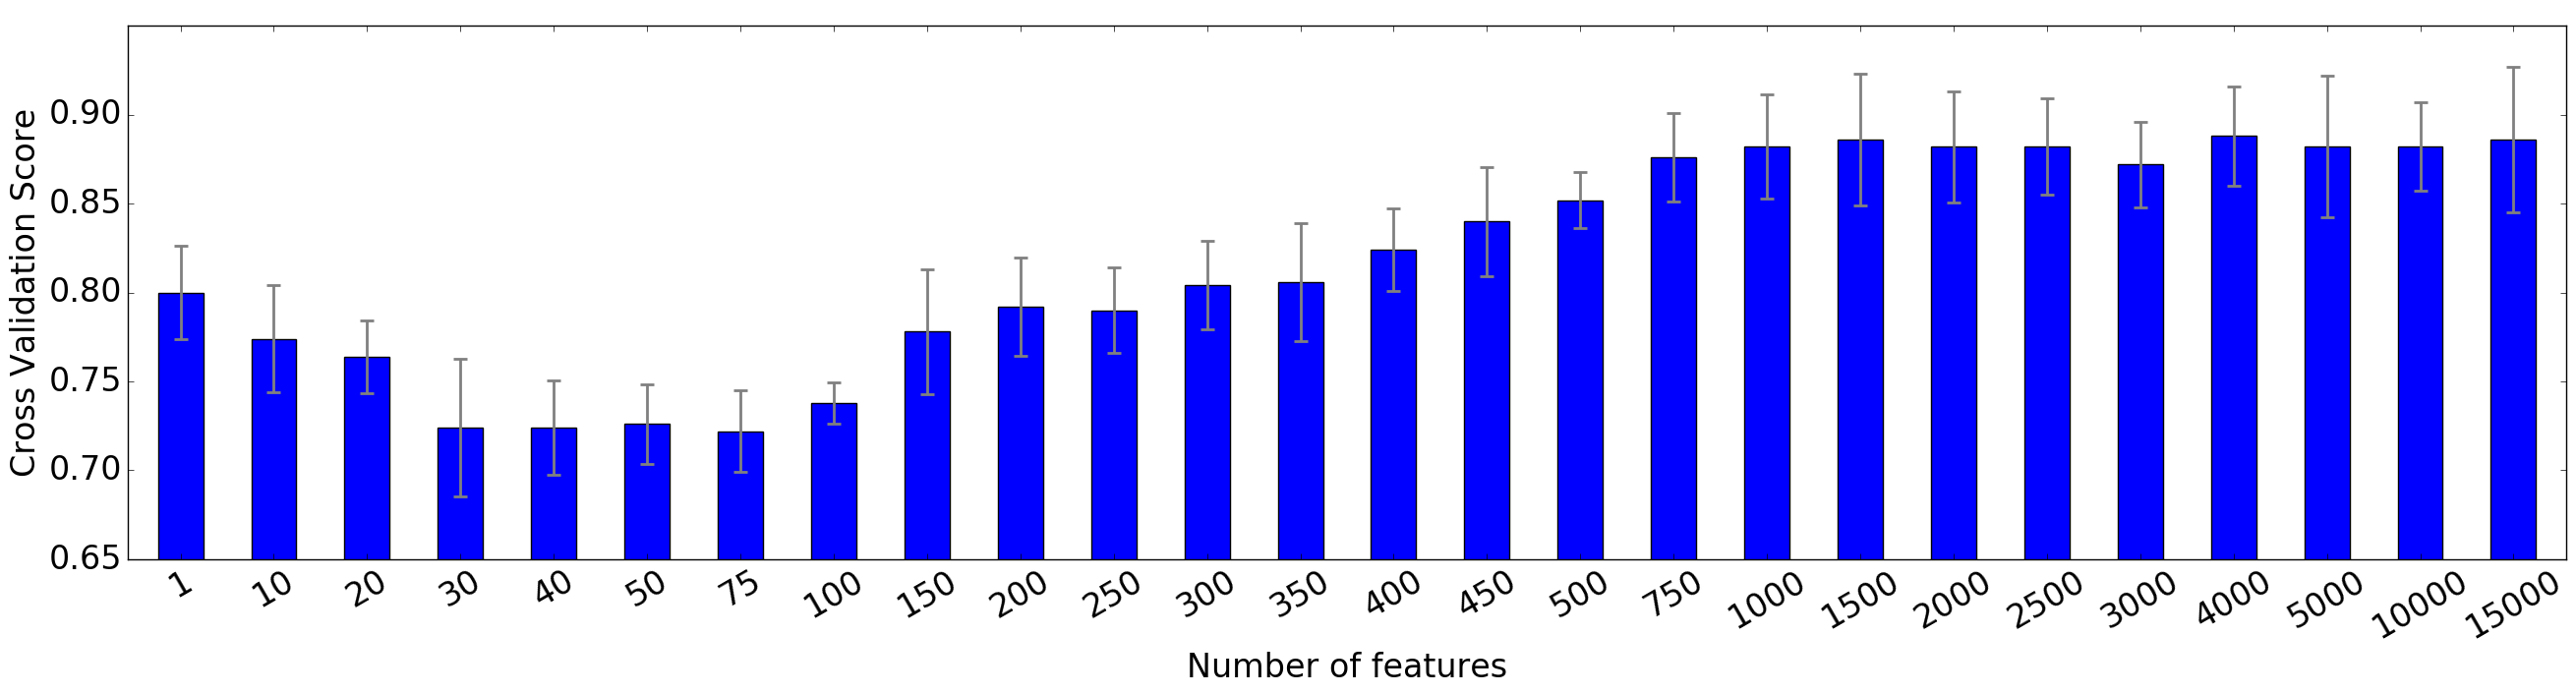
\includegraphics[width=1\textwidth]{report_images/num_features_vs_performance}
  \end{figure}

  Figure \ref{numfeatures} shows the mean 5-fold cross-validation scores and standard deviations for varying $n$. The peak performance is achieved with $n = 1000$. However its worth observing other values have margins of error that fall within the same score, also values between the shown bars were tested - the displayed bars are chosen for clarity. In choosing $n = 1000$ the resultantant classifier had a mean scores of 89\% with a standard deviation of 3\%, making it better than the majority class baseline by $9\%$.

  \section{Improving the Model}

  \subsection{Smarter Preprocessing}

  Several additional preprocessing techniques were implemented, the following paragraphs describe these techniques and give the associated accuracy values derived from soley applying that technique in conjunction with the previously detailed classifier of section \ref{baseline}.

  An initial flaw to observe about the simple preprocessing procedure described in section \ref{classconstr} is that the filtering of non purely-alphabetical substrings delimited by whitespace discriminates againsts words that appear next to punctuation, such as ``hello,'' or ``hello.''. This is counteracted by tokenizing the input string through matching to the regular expression ``$\backslash b \backslash w+ \backslash b$'', where $\backslash b$ matches to a word-boundary and $\backslash w$ matches to a alphabetical character. This change results in an improved score of 91\% accuracy.

  Another approach was to extract the content of the emails from the formatting of the emails. The emails were parsed to separate the headings and payload of the email, information from the subject header and the recipients fields was striped and concatenated to the content in the payload. Applying this technique in isolation gave an accuracy of 93\%.

  The third technique was numeric substitution, whereby numerical or alpha-numerical substrings would be replaced with the words ``num'' or ``alphanum''. The motivation for this was that numbers would often appear in emails, but the actual values in question wouldn't actually be semantically relevant. The hope of this substitution was to allow the system to better generalise. This gave an accuracy of 93\%.

  Similarly to numerical substitution was symbol processing - in most cases symbols were simply filtered out, however for symbols that provide meaning in their given contexts would be replaced with appropriate words, for example ``\$50'' would be replaced by `` money 50'' and ``cat \& dog '' would be replaced by ``cat and dog''. Substitutions would also be made when symbols appeared in sucession, such as ``free!!!'' being replaced with ``free multibang ''. Symbolic substitutions applied in isolation resulted in an accuracy of 92\%.


  The final technique was to process letter cases, any all-caps words such as ``OFFER'' were mapped to ``allcaps offer'', and everything else was converted to lowercase. This gave an accuracy of 91\%.

  The use of all of these methods in conjunction resulted in a mean 5-fold cross-validation score of 94\% with a 3\% standard devidation - a 5\% improvement from the simple preprocessing and a 14\% improvement from the baseline.


  % \subsection{Improved Feature Extraction}
  %


  \pagebreak

  \subsection{Optimising Classifier Hyperparameters} \label{hyperopt}

  \begin{wrapfigure}{R}{0.55\textwidth}
    \vspace{-0.6cm}
    \caption{Hyperparameter space}
    \vspace{-0.1cm}
    \label{hyperspace}
    \centering
    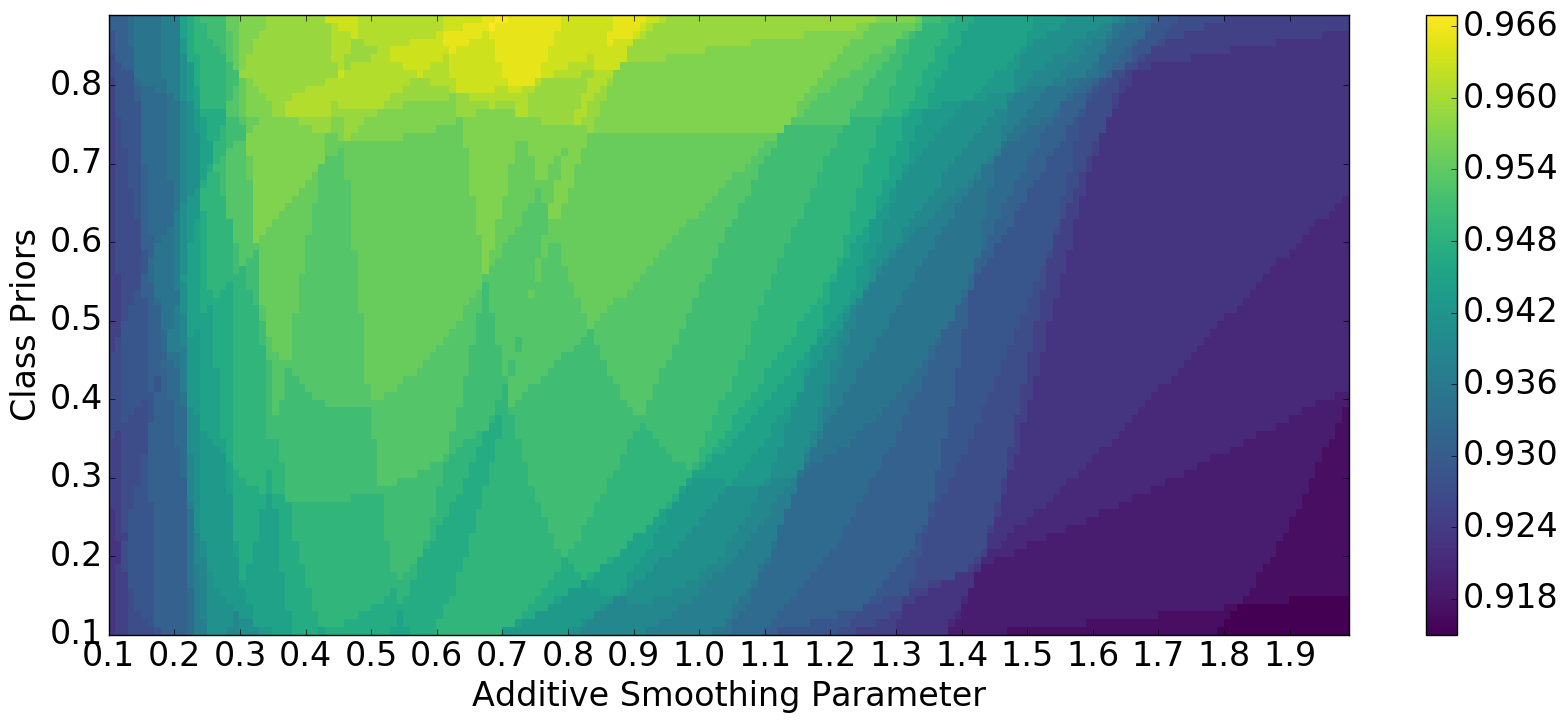
\includegraphics[width=1\linewidth]{report_images/MultinomialNB_param_space}
    \vspace{-1cm}
  \end{wrapfigure}

  In section \ref{classconstr} the hyperparameters $\alpha$ and $p$ of the Naive Bayes classifier were described. Figure \ref{hyperspace} visualises the three dimensional mapping $(\alpha, p) \mapsto s$ where $s$ is the mean 5-fold cross-validation score derived from the classifier constructed from the given parameters. The maxima on this surface is the point (0.7, 0.9), where the constructed classifer has an accuracy of 97\% with a standard deviation of 2\%.

  \subsection{Comparing to Another Classifier}



  \section{Extending the Model}

  \subsection{Calibration of Naive Bayes Probabilities}

  \subsection{Weighted Naive Bayes}

  Probability values were assigned to every word by dividing the total number of times the word appears across all the emails by the number of emails. More precisely for emails $e \in E$, let $f(e, w)$ detect the presence of a word in an email and $P(w | E)$ be the probabilty of a word appearing in an email.

  \vspace{-0.5cm}
  \begin{align*}
    f(e, w) &= \begin{cases}
      1   & \text{if } w \in e \\
      0   & \text{otherwise}
    \end{cases} \\
    \\
    \therefore P(w\ |\ E) &= \frac{1}{|E|}\sum_{e \in E}{f(e, w)}
  \end{align*}
  \vspace{-0.5cm}

  The motivation in constructing feature words was to look for the presence of words that best distinguished between spam and ham emails. Hence for the sets $S$ and $H$ of spam and ham emails a metric $d$ was devised to measure how well a given word differentiates between the classes:
  \vspace{-0.5cm}
  \begin{align*}
    d(w) = \max(|P(w\ |\ S)|,\ |P(w\ |\ H)|)
  \end{align*}
  Figure \ref{wordprobsham} plots this metric for the top thirty words across all the emails.

  \vspace{0.5cm}
  \begin{figure}[H]
    \caption{Top 30 most differentiating words}
    \label{wordprobsham}
    \vspace{-0.2cm}
    \centering
    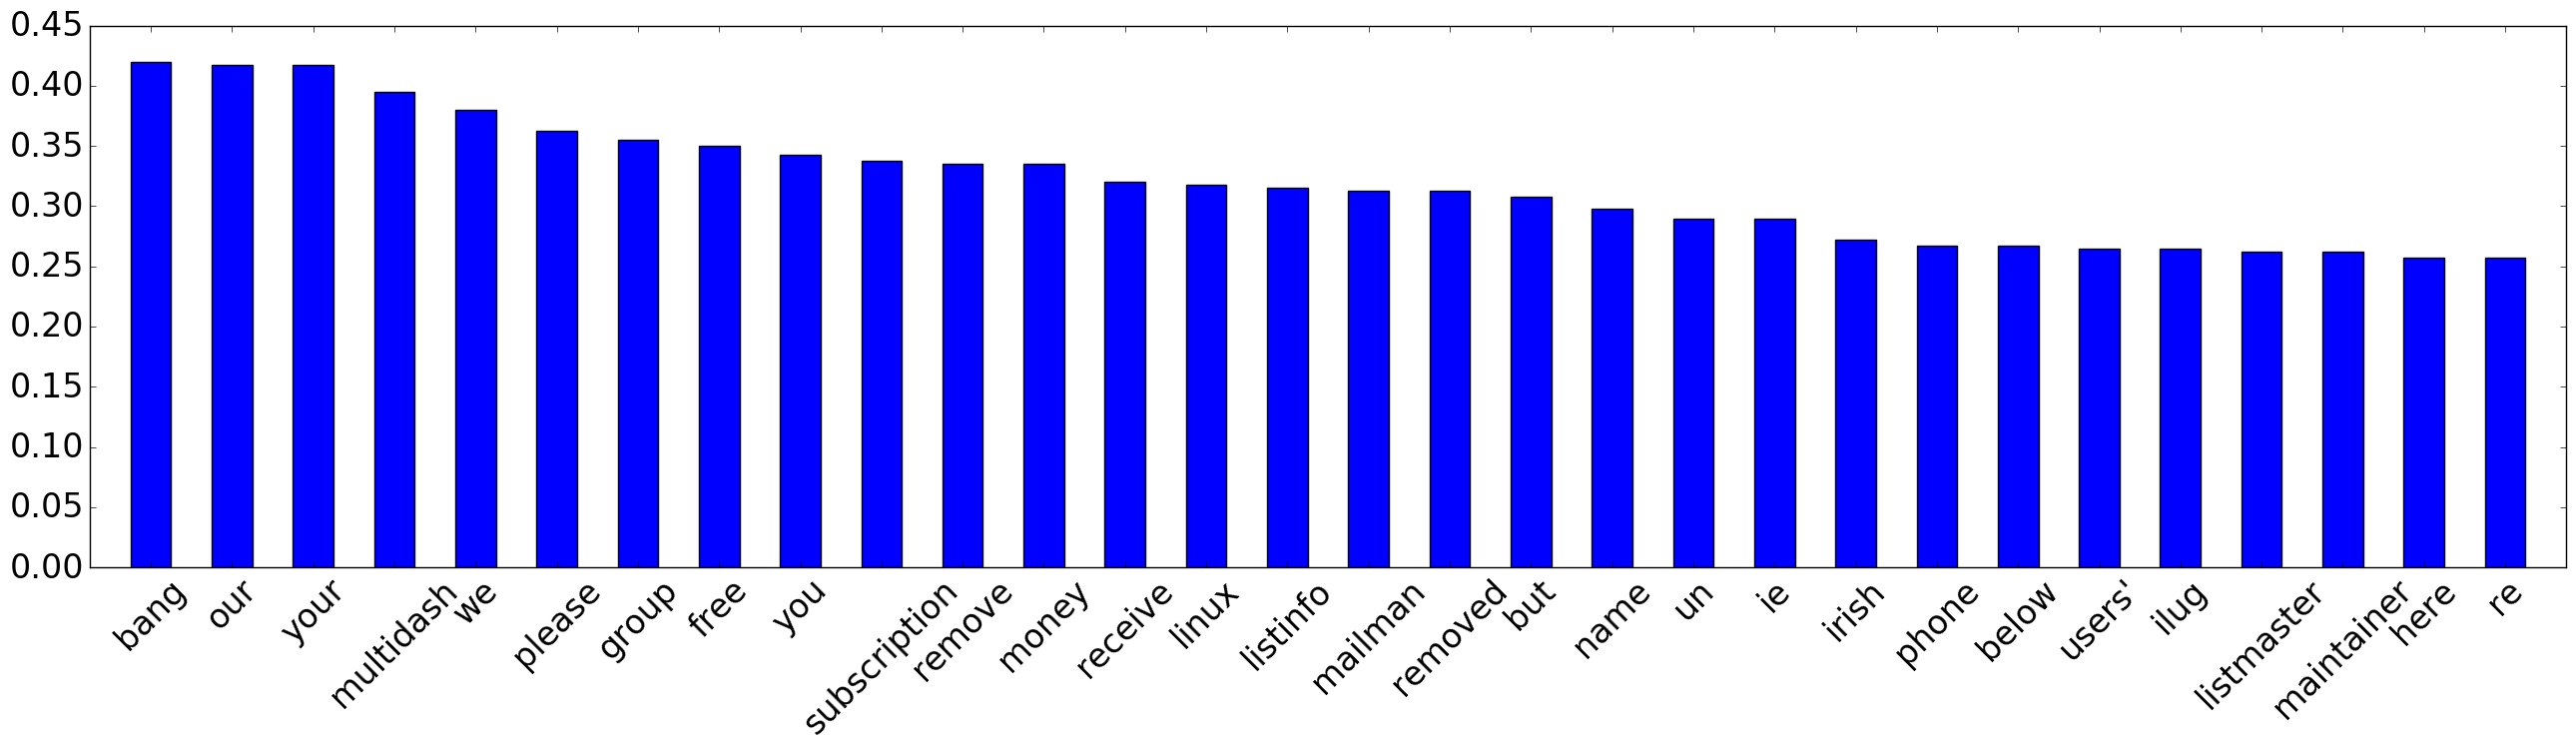
\includegraphics[width=1\linewidth]{report_images/word_probs_diff}
  \end{figure}

\end{document}
